\documentclass[twoside]{book}

% Packages required by doxygen
\usepackage{fixltx2e}
\usepackage{calc}
\usepackage{doxygen}
\usepackage[export]{adjustbox} % also loads graphicx
\usepackage{graphicx}
\usepackage[utf8]{inputenc}
\usepackage{makeidx}
\usepackage{multicol}
\usepackage{multirow}
\PassOptionsToPackage{warn}{textcomp}
\usepackage{textcomp}
\usepackage[nointegrals]{wasysym}
\usepackage[table]{xcolor}

% Font selection
\usepackage[T1]{fontenc}
\usepackage[scaled=.90]{helvet}
\usepackage{courier}
\usepackage{amssymb}
\usepackage{sectsty}
\renewcommand{\familydefault}{\sfdefault}
\allsectionsfont{%
  \fontseries{bc}\selectfont%
  \color{darkgray}%
}
\renewcommand{\DoxyLabelFont}{%
  \fontseries{bc}\selectfont%
  \color{darkgray}%
}
\newcommand{\+}{\discretionary{\mbox{\scriptsize$\hookleftarrow$}}{}{}}

% Page & text layout
\usepackage{geometry}
\geometry{%
  a4paper,%
  top=2.5cm,%
  bottom=2.5cm,%
  left=2.5cm,%
  right=2.5cm%
}
\tolerance=750
\hfuzz=15pt
\hbadness=750
\setlength{\emergencystretch}{15pt}
\setlength{\parindent}{0cm}
\setlength{\parskip}{3ex plus 2ex minus 2ex}
\makeatletter
\renewcommand{\paragraph}{%
  \@startsection{paragraph}{4}{0ex}{-1.0ex}{1.0ex}{%
    \normalfont\normalsize\bfseries\SS@parafont%
  }%
}
\renewcommand{\subparagraph}{%
  \@startsection{subparagraph}{5}{0ex}{-1.0ex}{1.0ex}{%
    \normalfont\normalsize\bfseries\SS@subparafont%
  }%
}
\makeatother

% Headers & footers
\usepackage{fancyhdr}
\pagestyle{fancyplain}
\fancyhead[LE]{\fancyplain{}{\bfseries\thepage}}
\fancyhead[CE]{\fancyplain{}{}}
\fancyhead[RE]{\fancyplain{}{\bfseries\leftmark}}
\fancyhead[LO]{\fancyplain{}{\bfseries\rightmark}}
\fancyhead[CO]{\fancyplain{}{}}
\fancyhead[RO]{\fancyplain{}{\bfseries\thepage}}
\fancyfoot[LE]{\fancyplain{}{}}
\fancyfoot[CE]{\fancyplain{}{}}
\fancyfoot[RE]{\fancyplain{}{\bfseries\scriptsize Generated by Doxygen }}
\fancyfoot[LO]{\fancyplain{}{\bfseries\scriptsize Generated by Doxygen }}
\fancyfoot[CO]{\fancyplain{}{}}
\fancyfoot[RO]{\fancyplain{}{}}
\renewcommand{\footrulewidth}{0.4pt}
\renewcommand{\chaptermark}[1]{%
  \markboth{#1}{}%
}
\renewcommand{\sectionmark}[1]{%
  \markright{\thesection\ #1}%
}

% Indices & bibliography
\usepackage{natbib}
\usepackage[titles]{tocloft}
\setcounter{tocdepth}{3}
\setcounter{secnumdepth}{5}
\makeindex

% Hyperlinks (required, but should be loaded last)
\usepackage{ifpdf}
\ifpdf
  \usepackage[pdftex,pagebackref=true]{hyperref}
\else
  \usepackage[ps2pdf,pagebackref=true]{hyperref}
\fi
\hypersetup{%
  colorlinks=true,%
  linkcolor=blue,%
  citecolor=blue,%
  unicode%
}

% Custom commands
\newcommand{\clearemptydoublepage}{%
  \newpage{\pagestyle{empty}\cleardoublepage}%
}

\usepackage{caption}
\captionsetup{labelsep=space,justification=centering,font={bf},singlelinecheck=off,skip=4pt,position=top}

%===== C O N T E N T S =====

\begin{document}

% Titlepage & ToC
\hypersetup{pageanchor=false,
             bookmarksnumbered=true,
             pdfencoding=unicode
            }
\pagenumbering{alph}
\begin{titlepage}
\vspace*{7cm}
\begin{center}%
{\Large My Project }\\
\vspace*{1cm}
{\large Generated by Doxygen 1.8.14}\\
\end{center}
\end{titlepage}
\clearemptydoublepage
\pagenumbering{roman}
\tableofcontents
\clearemptydoublepage
\pagenumbering{arabic}
\hypersetup{pageanchor=true}

%--- Begin generated contents ---
\chapter{Line\+Threshold Library}
\label{md__r_e_a_d_m_e}
\Hypertarget{md__r_e_a_d_m_e}

\begin{DoxyItemize}
\item A library that uses calclates thresholds to know what region the robot line sensors are over
\begin{DoxyItemize}
\item It is designed to work on the \href{https://www.pololu.com/product/2506}{\tt Z\+U\+MO robot for arduino} using the \href{https://www.arduino.cc/en/Main/Software}{\tt Arduino Integrated Development Enviornment}
\end{DoxyItemize}
\item The functions are outlined in the header file ~\newline
 + They allow the robot to determine what region it is over
\begin{DoxyItemize}
\item given an array of region names and thresholds, as well as an array of the priority of regions -\/\+The Brandeis University Robotics Club  
\end{DoxyItemize}
\end{DoxyItemize}
\chapter{Hierarchical Index}
\section{Class Hierarchy}
This inheritance list is sorted roughly, but not completely, alphabetically\+:\begin{DoxyCompactList}
\item Line\+Shield\begin{DoxyCompactList}
\item \contentsline{section}{Line\+Threshold}{\pageref{class_line_threshold}}{}
\end{DoxyCompactList}
\end{DoxyCompactList}

\chapter{Class Index}
\section{Class List}
Here are the classes, structs, unions and interfaces with brief descriptions\+:\begin{DoxyCompactList}
\item\contentsline{section}{\mbox{\hyperlink{class_line_threshold}{Line\+Threshold}} }{\pageref{class_line_threshold}}{}
\end{DoxyCompactList}

\chapter{Class Documentation}
\hypertarget{class_line_threshold}{}\section{Line\+Threshold Class Reference}
\label{class_line_threshold}\index{Line\+Threshold@{Line\+Threshold}}
Inheritance diagram for Line\+Threshold\+:\begin{figure}[H]
\begin{center}
\leavevmode
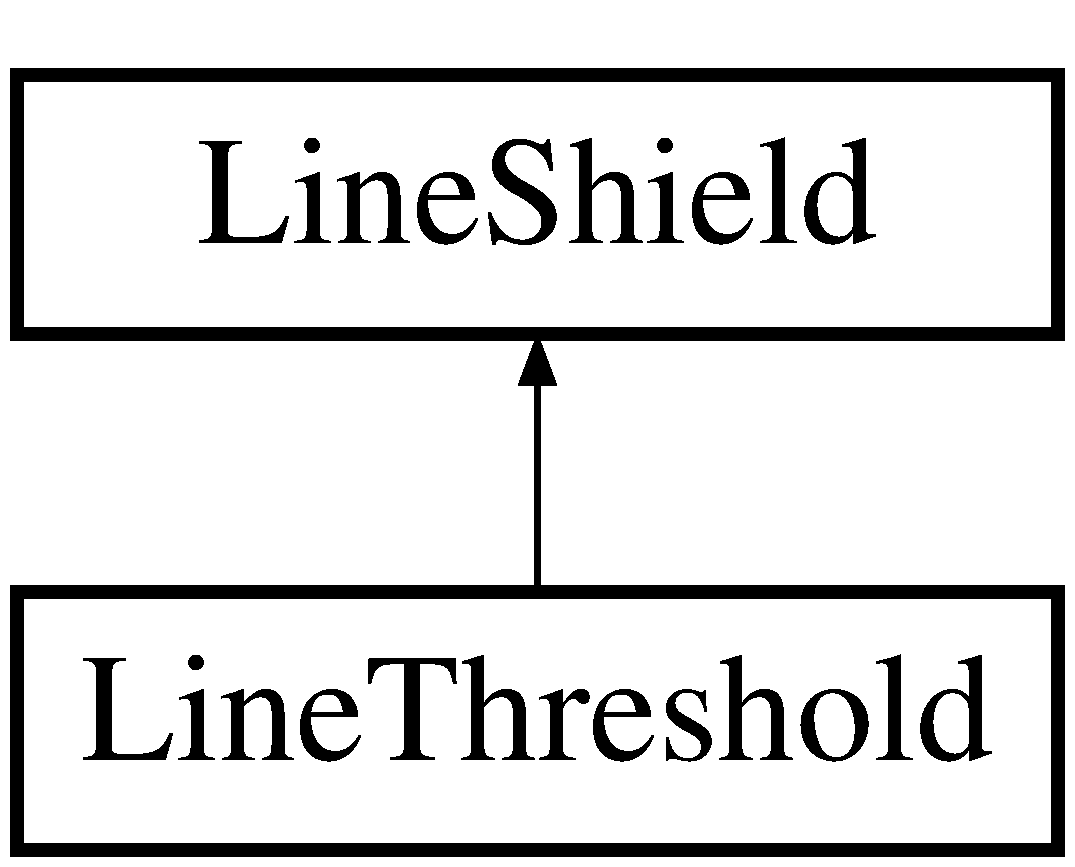
\includegraphics[height=2.000000cm]{class_line_threshold}
\end{center}
\end{figure}
\subsection*{Public Member Functions}
\begin{DoxyCompactItemize}
\item 
\mbox{\hyperlink{class_line_threshold_a927e9c11dcec815c2e64d6ea7202c3fb}{Line\+Threshold}} (int $\ast$region\+Thresholds, String $\ast$regions, String $\ast$regions\+Priority, int num\+Regions, String $\ast$regions\+Seen)
\item 
String \mbox{\hyperlink{class_line_threshold_a57c6827535c3cd2611f93f7e52e3ec95}{get\+Region}} ()
\end{DoxyCompactItemize}


\subsection{Constructor \& Destructor Documentation}
\mbox{\Hypertarget{class_line_threshold_a927e9c11dcec815c2e64d6ea7202c3fb}\label{class_line_threshold_a927e9c11dcec815c2e64d6ea7202c3fb}} 
\index{Line\+Threshold@{Line\+Threshold}!Line\+Threshold@{Line\+Threshold}}
\index{Line\+Threshold@{Line\+Threshold}!Line\+Threshold@{Line\+Threshold}}
\subsubsection{\texorpdfstring{Line\+Threshold()}{LineThreshold()}}
{\footnotesize\ttfamily Line\+Threshold\+::\+Line\+Threshold (\begin{DoxyParamCaption}\item[{int $\ast$}]{region\+Thresholds,  }\item[{String $\ast$}]{regions,  }\item[{String $\ast$}]{regions\+Priority,  }\item[{int}]{num\+Regions,  }\item[{String $\ast$}]{regions\+Seen }\end{DoxyParamCaption})}

creates a new Line\+Shield\+Shield object with defual sensor reading

//creates a new \mbox{\hyperlink{class_line_threshold}{Line\+Threshold}} object with dual sensor reading 
\begin{DoxyParams}{Parameters}
{\em region\+Thresholds} & an array of the brightness readings that divide regions \\
\hline
{\em regions} & an array of the name of regions in order of thresholds \\
\hline
{\em regions\+Priority} & an array of the name of regions in order of their priority \\
\hline
{\em num\+Regions} & the number of regions \\
\hline
{\em regions\+Seen} & an array of the regions the line sensors have seen to be populated \\
\hline
\end{DoxyParams}


\subsection{Member Function Documentation}
\mbox{\Hypertarget{class_line_threshold_a57c6827535c3cd2611f93f7e52e3ec95}\label{class_line_threshold_a57c6827535c3cd2611f93f7e52e3ec95}} 
\index{Line\+Threshold@{Line\+Threshold}!get\+Region@{get\+Region}}
\index{get\+Region@{get\+Region}!Line\+Threshold@{Line\+Threshold}}
\subsubsection{\texorpdfstring{get\+Region()}{getRegion()}}
{\footnotesize\ttfamily String Line\+Threshold\+::get\+Region (\begin{DoxyParamCaption}{ }\end{DoxyParamCaption})}

returns the region the robot is in

\begin{DoxyReturn}{Returns}
the region the robot is on 
\end{DoxyReturn}


The documentation for this class was generated from the following files\+:\begin{DoxyCompactItemize}
\item 
Line\+Threshold.\+h\item 
Line\+Threshold.\+cpp\end{DoxyCompactItemize}

%--- End generated contents ---

% Index
\backmatter
\newpage
\phantomsection
\clearemptydoublepage
\addcontentsline{toc}{chapter}{Index}
\printindex

\end{document}
